\subsection{Forma del fascio}

Abbiamo fatto delle misure di conteggio a vari angoli con e senza collimatori per studiare la forma del fascio.

\subsubsection{Assenza di collimatori}

La misura in assenza di collimatori ci permette di indagare la forma del fascio di particelle $\alpha$ in uscita dalla sorgente di \am{}.
\marginpar{disegno provvisorio}
Bisogna notare che l'angolo segnato sulla scala graduata non coincide con quello tra la sorgente ed il rivelatore perché il fotodiodo non è al centro della camera a vuoto, inoltre all'aumentare (in modulo) dell'angolo la distanza tra sorgente e rivelatore diminuisce. 
Lo schema di \autoref{fma} illustra la situazione.

\begin{figure}[h]
\centering
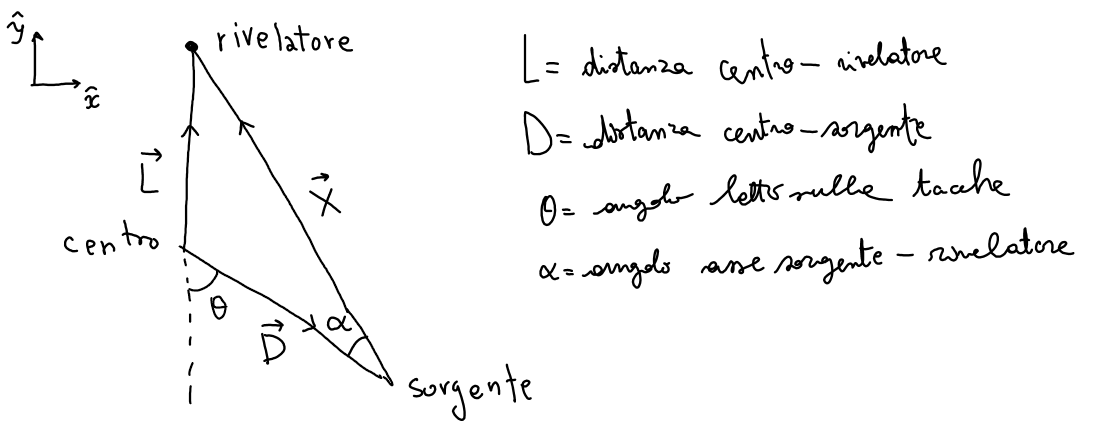
\includegraphics[width=30 em]{immagini/fma_provv}
\caption{Schema raffigurante gli angoli tra rivelatore, centro della camera a vuoto e sorgente.}
\label{fma}
\end{figure}

Applicate le dovute correzioni e usando le variabili di \autoref{fma} troviamo che l'angolo tra rivelatore e sorgente è
\begin{equation}
\cos{\alpha}= -\frac{\vec{X} \cdot \vec{D} }{ |\vec{X}| |\vec{D}| } = \frac{ L \cos{\theta} + D }{ \sqrt{ L^2+2LD\cos{\theta}+D^2  } }.
\end{equation}

Teniamo conto della variazione della distanza al variare dell'angolo moltiplicando ogni rate per $|\vec{X}|^2$.
Tale fattore è giustificato dal fatto che supponiamo isotropa l'emissione di particelle $\alpha$ da parte della sorgente.
Se $C$ è una costante, abbiamo che $$ \frac{dN}{d^3r}=C \implies \frac{dN}{dr}=C 4\pi r^2. $$

In virtù delle precedenti affermazioni, abbiamo calcolato il rate in \si{s^{-1}cm^2}.

Il risultato di questa misura è presente in \autoref{fig:forma}, invece la \autoref{tab:forma} contiene i dati di tale grafico.
Si evince che il fascio ha un'estensione angolare di quasi \SI{50}{\degree}. 

\begin{figure}[h]
\centering
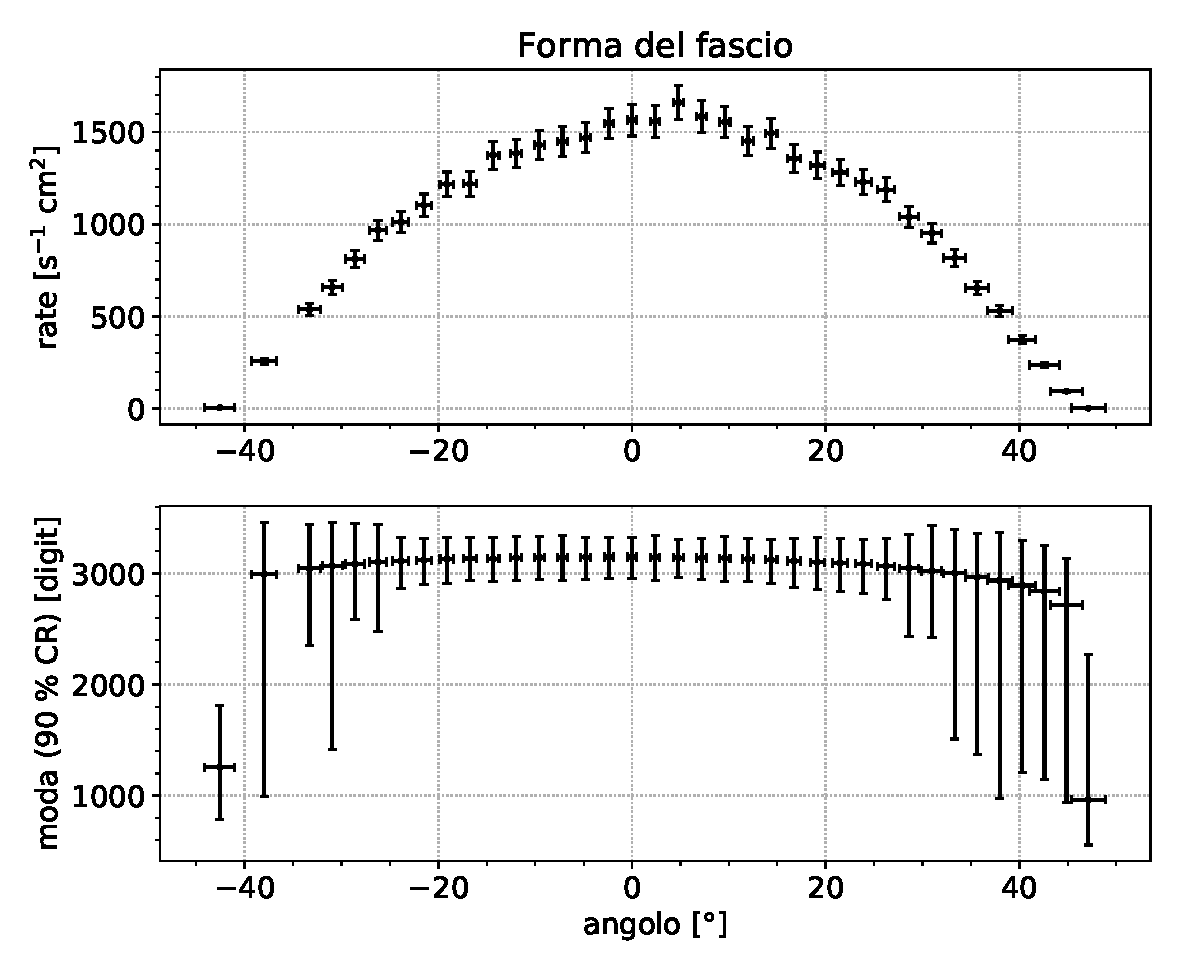
\includegraphics[width=30 em]{immagini/forma}
\caption{Grafico rappresentante la forma del fascio. Nel pannello superiore è presente l'estensione angolare del fascio estrapolata dai conteggi, in quello inferiore sono presenti le mode dei relativi istogrammi.}
\label{fig:forma}
\end{figure}

\begin{table}[h]
\centering

\begin{tabular}{c|c|c}
angolo [\si{\degree}] & rate  [\si{s^{-1}cm^2}] & moda [digit] \\
\hline
$ -42.6 \pm 1.5 $ & $ 5.2 \pm 1.3 $ & $ 1256 $ \\ 
$ -38.0 \pm 1.3 $ & $ 257 \pm 16 $ & $ 2993 $ \\ 
$ -33.3 \pm 1.1 $ & $ 538 \pm 31 $ & $ 3048 $ \\ 
$ -31.0 \pm 1.0 $ & $ 6.6 \pm 0.4   \cdot 10^{2} $ & $ 3070 $ \\ 
$ -28.6 \pm 1.0 $ & $ 8.1 \pm 0.5   \cdot 10^{2} $ & $ 3087 $ \\ 
$ -26.2 \pm 0.9 $ & $ 9.7 \pm 0.5   \cdot 10^{2} $ & $ 3105 $ \\ 
$ -23.9 \pm 0.8 $ & $ 1.01 \pm 0.06 \cdot 10^{3} $ & $ 3113 $ \\ 
$ -21.5 \pm 0.8 $ & $ 1.10 \pm 0.06 \cdot 10^{3} $ & $ 3119 $ \\ 
$ -19.1 \pm 0.7 $ & $ 1.22 \pm 0.07 \cdot 10^{3} $ & $ 3129 $ \\ 
$ -16.7 \pm 0.7 $ & $ 1.22 \pm 0.07 \cdot 10^{3} $ & $ 3135 $ \\ 
$ -14.4 \pm 0.6 $ & $ 1.37 \pm 0.08 \cdot 10^{3} $ & $ 3134 $ \\ 
$ -12.0 \pm 0.6 $ & $ 1.39 \pm 0.08 \cdot 10^{3} $ & $ 3142 $ \\ 
$ -9.6 \pm 0.5 $ & $ 1.43 \pm 0.08  \cdot 10^{3} $ & $ 3144 $ \\ 
$ -7.2 \pm 0.5 $ & $ 1.45 \pm 0.08  \cdot 10^{3} $ & $ 3147 $ \\ 
$ -4.8 \pm 0.5 $ & $ 1.47 \pm 0.08  \cdot 10^{3} $ & $ 3145 $ \\ 
$ -2.4 \pm 0.5 $ & $ 1.55 \pm 0.08  \cdot 10^{3} $ & $ 3148 $ \\ 
$ 0.0 \pm 0.5 $ & $ 1.56 \pm 0.09   \cdot 10^{3} $ & $ 3149 $ \\ 
$ 2.4 \pm 0.5 $ & $ 1.56 \pm 0.09   \cdot 10^{3} $ & $ 3145 $ \\ 
$ 4.8 \pm 0.5 $ & $ 1.66 \pm 0.09   \cdot 10^{3} $ & $ 3141 $ \\ 
$ 7.2 \pm 0.5 $ & $ 1.59 \pm 0.09   \cdot 10^{3} $ & $ 3140 $ \\ 
$ 9.6 \pm 0.5 $ & $ 1.56 \pm 0.09   \cdot 10^{3} $ & $ 3137 $ \\ 
$ 12.0 \pm 0.6 $ & $ 1.45 \pm 0.08  \cdot 10^{3} $ & $ 3130 $ \\ 
$ 14.4 \pm 0.6 $ & $ 1.49 \pm 0.08  \cdot 10^{3} $ & $ 3125 $ \\ 
$ 16.7 \pm 0.7 $ & $ 1.36 \pm 0.08  \cdot 10^{3} $ & $ 3114 $ \\ 
$ 19.1 \pm 0.7 $ & $ 1.32 \pm 0.07  \cdot 10^{3} $ & $ 3101 $ \\ 
$ 21.5 \pm 0.8 $ & $ 1.28 \pm 0.07  \cdot 10^{3} $ & $ 3095 $ \\ 
$ 23.9 \pm 0.8 $ & $ 1.23 \pm 0.07  \cdot 10^{3} $ & $ 3087 $ \\ 
$ 26.2 \pm 0.9 $ & $ 1.19 \pm 0.07  \cdot 10^{3} $ & $ 3066 $ \\ 
$ 28.6 \pm 1.0 $ & $ 1.04 \pm 0.06  \cdot 10^{3} $ & $ 3047 $ \\ 
$ 31.0 \pm 1.0 $ & $ 9.5 \pm 0.5    \cdot 10^{2} $ & $ 3022 $ \\ 
$ 33.3 \pm 1.1 $ & $ 8.2 \pm 0.5    \cdot 10^{2} $ & $ 3002 $ \\ 
$ 35.7 \pm 1.2 $ & $ 6.5 \pm 0.4    \cdot 10^{2} $ & $ 2966 $ \\ 
$ 38.0 \pm 1.3 $ & $ 531 \pm 30 $ & $ 2937 $ \\ 
$ 40.3 \pm 1.4 $ & $ 374 \pm 21 $ & $ 2892 $ \\ 
$ 42.6 \pm 1.5 $ & $ 237 \pm 14 $ & $ 2840 $ \\ 
$ 44.9 \pm 1.6 $ & $ 94 \pm 6 $ & $ 2717 $ \\ 
$ 47.1 \pm 1.8 $ & $ 2.6 \pm 0.9 $ & $ 964 $ \\ 
\end{tabular}

\caption{Dati utilizzati per trovare la forma del fascio. L'errore sulla moda è dato dal 90\% di credibilità del relativo istogramma.}
\label{tab:forma}
\end{table}

Useremo queste informazioni (se sarà necessario) nell'analizzare i dati sulla sezione d'urto.

\subsubsection{Collimatore da 5\! mm}

Analizziamo la forma del fascio con un collimatore da \SI{5}{mm} che ci dà un errore minore sull'angolo di incidenza delle particelle $\alpha$.
Con i dati presenti in \autoref{tab:coll5} abbiamo il grafico di \autoref{fig:coll5}.

In questo caso i conteggi sono non nulli soltanto nell'intervallo \SI{\mp10}{\degree}. La parte piatta al centro del grafico è dovuta all'effetto descritto nella sezione precedente (non corretto), ancora visibile con un'apertura di tale larghezza.

\begin{figure}[h]
\centering
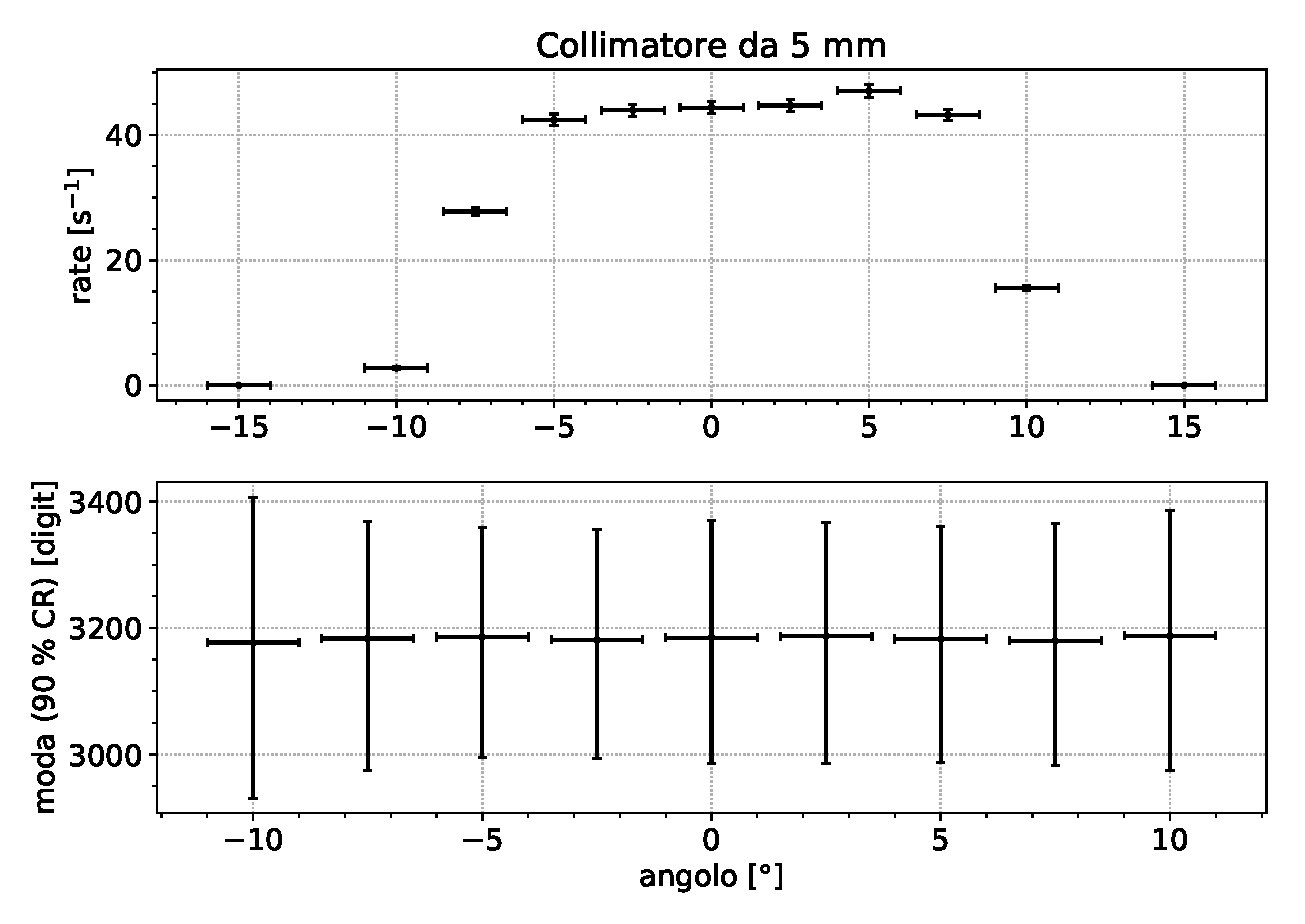
\includegraphics[width=30 em]{immagini/coll5}
\caption{Grafico del rate in funzione dell'angolo con il collimatore da 5\! mm.}
\label{fig:coll5}
\end{figure}

\begin{table}[h]
\centering

\begin{tabular}{c|c|c}
angolo [\si{\degree}] & rate  [\si{s^{-1}}] & moda [digit] \\
\hline
$ -15.00 $ & $ 0.0 \pm 0 $ & $ 0 $ \\ 
$ -10.00 $ & $ 2.76 \pm 0.18 $ & $ 3177 $ \\ 
$ -7.50 $ & $ 27.8 \pm 0.6 $ & $ 3183 $ \\ 
$ -5.00 $ & $ 42.4 \pm 0.9 $ & $ 3186 $ \\ 
$ -2.50 $ & $ 43.9 \pm 1.0 $ & $ 3181 $ \\ 
$ 0.00 $ & $ 44.4 \pm 0.9 $ & $ 3185 $ \\ 
$ 2.50 $ & $ 44.7 \pm 1.0 $ & $ 3187 $ \\ 
$ 5.00 $ & $ 47.1 \pm 1.0 $ & $ 3182 $ \\ 
$ 7.50 $ & $ 43.2 \pm 0.9 $ & $ 3180 $ \\ 
$ 10.00 $ & $ 15.6 \pm 0.4 $ & $ 3188 $ \\ 
$ 15.00 $ & $ 0.0 \pm 0 $ & $ 0 $ \\ 

\end{tabular}

\caption{Rate in funzione dell'angolo con il collimatore da 5\! mm.
		L'errore sugli angoli è stimato essere 1.25$^{\circ}$.}
\label{tab:coll5}
\end{table}

\subsubsection{Collimatore da 1\! mm}

Studiamo la forma del fascio con il collimatore da \SI1{mm} che ci permette di avere il più piccolo errore possibile sull'angolo di incidenza.
Di contro abbiamo un rate minore che nei casi precedenti.
I dati presenti in \autoref{tab:coll1} e \autoref{fig:coll1} sono stati analizzati come in precedenza.
Stavolta abbiamo conteggi solo in un intervallo di \SI{5}{\degree}.

\begin{table}[h]
\centering

\begin{tabular}{c|c|c}
angolo [\si{\degree}] & rate  [\si{s^{-1}}] & moda [digit] \\
\hline
$ -2.50 $ & $ 0.08 \pm 0.04 $ & $ 3156 $ \\ 
$ -1.25 $ & $ 2.48 \pm 0.20 $ & $ 3171 $ \\ 
$ 0.00 $ & $ 14.63 \pm 0.32 $ & $ 3174 $ \\ 
$ 1.25 $ & $ 31.5 \pm 0.7 $ & $ 3178 $ \\ 
$ 2.50 $ & $ 34.8 \pm 0.8 $ & $ 3185 $ \\ 
$ 3.75 $ & $ 26.9 \pm 0.6 $ & $ 3184 $ \\ 
$ 5.00 $ & $ 12.70 \pm 0.31 $ & $ 3188 $ \\ 
$ 6.25 $ & $ 2.81 \pm 0.22 $ & $ 3193 $ \\ 
$ 7.50 $ & $ 0.11 \pm 0.04 $ & $ 3185 $ \\ 

\end{tabular}

\caption{Dati per le misure con il collimatore da 1\! mm.}
\label{tab:coll1}
\end{table}


\begin{figure}[h]
\centering
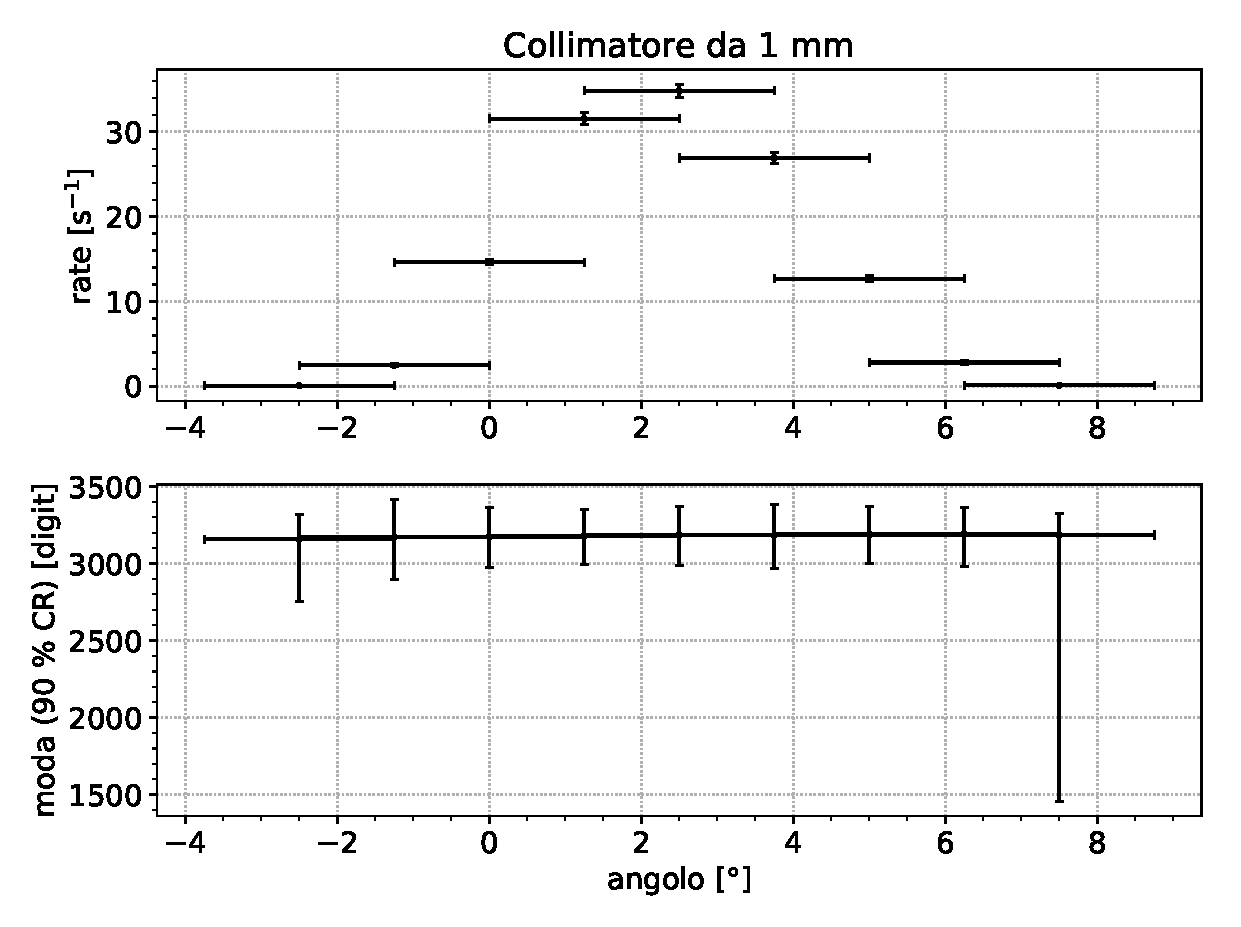
\includegraphics[width=30 em]{immagini/coll1}
\caption{Grafico del rate in funzione dell'angolo con il collimatore da 1\! mm.}
\label{fig:coll1}
\end{figure}

\subsubsection{Collimatore a croce}

Cerchiamo infine di collimare il fascio il più possibile sovrapponendo 2 collimatori da \SI1{mm} di cui uno ruotato di \SI{90}{\degree} rispetto all'altro. In questo modo abbiamo una piccola finestra che seleziona le particelle sia verticalmente che orizzontalmente.
Prendiamo le misure in \autoref{tab:super} e guardiamo il grafico di \autoref{fig:super}.

\begin{table}
\centering

\begin{tabular}{c|c|c}
angolo [\si{\degree}] & rate  [\si{s^{-1}}] & moda [digit] \\
\hline
$ -2.50 $ & $ 0.27 \pm 0.04 $ & $ 3213 $ \\ 
$ -1.25 $ & $ 1.20 \pm 0.11 $ & $ 3198 $ \\ 
$ 0.00 $ & $ 2.36 \pm 0.15 $ & $ 3190 $ \\ 
$ 1.25 $ & $ 2.56 \pm 0.16 $ & $ 3187 $ \\ 
$ 2.50 $ & $ 2.41 \pm 0.15 $ & $ 3192 $ \\ 
$ 3.75 $ & $ 1.32 \pm 0.09 $ & $ 3187 $ \\ 
$ 5.00 $ & $ 0.32 \pm 0.05 $ & $ 3193 $ \\ 

\end{tabular}

\caption{Dati per le misure con il collimatore a croce.}
\label{tab:super}
\end{table}

\begin{figure}[h]
\centering
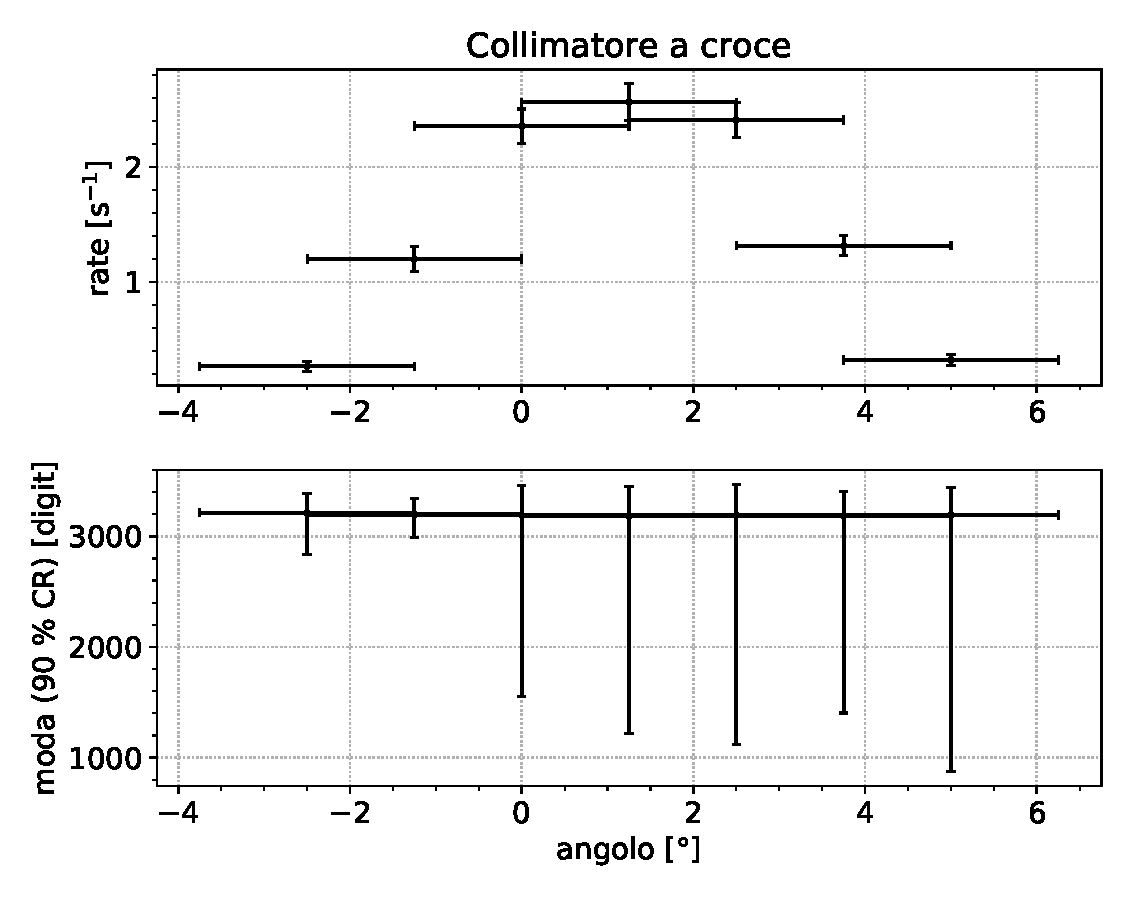
\includegraphics[width=30 em]{immagini/supercoll}
\caption{Grafico del rate in funzione dell'angolo con il collimatore a croce.}
\label{fig:super}
\end{figure}

Questa configurazione è ottimale per avere un fascio collimato, ma non la useremo a causa del rate incredibilmente basso.



